\subsection{Axon-hillock circuit}

How can we model the behaviour of cortical neurons, i.e. their ability to generate an action potential when the sum of the synaptic inputs reaches a certain threshold, with a minimal circuit to reduce the negative impact of device mismatch? One such circuit (which you should be able to explain at the exam) is the Axon-hillock circuit. It is an integrate-and-fire neuron model that was proposed by Carver Mead in the late 1980s. It has positive feedback (similar to sodium in neurons), negative feedback (similar to potassium), and a membrane capacitance. The circuit schematic is shown in figure \ref{fig:axonHillockCircuit}. The amplifier acts as a comparator between its input voltage $V_{mem}$ and a threshold voltage $V_{th}$ that is not explicitly denoted in the schematic.\\

\begin{figure}
    \centering
    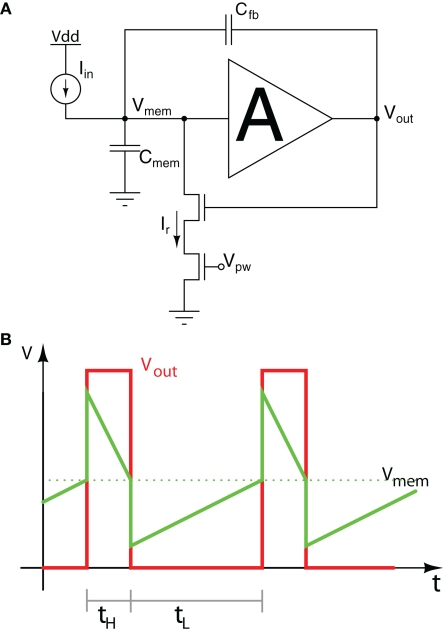
\includegraphics[width=.6\linewidth]{Figures/Axon_hillock_circuit.png}
    \caption{Axon hillock circuit.}
    \label{fig:axonHillockCircuit}
\end{figure}

The behavior of the Axon-hillock circuit can be explained as follows:

\begin{enumerate}
    \item At the beginning, we don't have any input current and our membrane potential $V_{mem}$ is zero. Consequently, our non-inverting amplifier also has a zero output voltage which acts as the gate voltage of the reset transistor that is turned off. For now, we ignore the positive feedback component of the circuit.
    \item With constant input current, the increase in charge at the capacitor $C_mem$ leads to a linear increase of $V_{mem}$.
    \item When $V_{mem}$ crosses the threshold voltage $V_{thr}$ of the amplifier, the output $V_out$ will go from zero to $V_{dd}$. We now have a positive gate voltage that turns on our reset transistor and generate a current $I_r$.
    \item With $I_r$ larger than $I_{in}$, the capacitor discharges and $V_{mem}$ decreases again until the amplifier switches off, which turns $V_{out}$ back to zero. Consequently, the current $I_r$ become zero again and the charging of the membrane voltage restarts.
\end{enumerate}

In reality, however, our $V_{mem}$ is not in- or decreasing perfectly linearly but is distorted by noise. When it comes close to the threshold, the noise causes the membrane voltage to fluctuate below and above threshold and therefore leading to a fluctuating output voltage as well. How can we prevent these fluctuations from happening? By introducing an additional capacitor to the circuit which acts as a positive feedback, we are able to make our membrane voltage more robust towards noise.\\

\begin{figure}
    \centering
    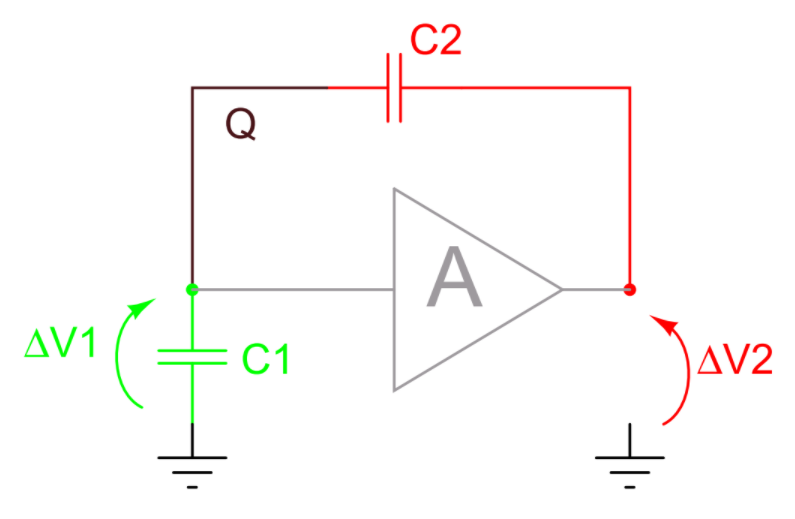
\includegraphics[width=.6\linewidth]{Figures/axon_hillock_capacitive_divider.PNG}
    \caption{Capacitive divider within the Axon Hillock circuit.}
    \label{fig:axon_hillock_capacitive_divider}
\end{figure}

But how exactly does the positive feedback work? By adding a second capacitor, we get a capacitive divider circuit as shown in figure \ref{fig:axon_hillock_capacitive_divider}. Assuming that the charge within the circuit is constant, the following equation describes our circuit:

\begin{equation}
    Q = C_1 V_1 + C_2 (V_1 - V_2) = constant
\end{equation}

We are interested in the circuit's behaviour when our voltage changes, as is the case when our output voltage jumps to $V_{dd}$ once we cross the threshold voltage. With $\Delta Q = 0$ for a constant $Q$, we get:

\begin{equation}
    C_1 \Delta V_1 + C_2 (\Delta V_1 - \Delta V_2) = 0
\end{equation}

\begin{equation}
    \Delta V_1 = \frac{C_2}{C_1 + C_2} \Delta V_2
\end{equation}

\begin{equation}
    \Delta V_{mem} = \frac{C_{fb}}{C_m + C_{fb}} V_{dd} \label{eq:positive_feedback}
\end{equation}

The positive feedback inserted back into our membrane voltage corresponds to a fraction of $V_{dd}$ as shown in \eqref{eq:positive_feedback}. Thanks to our positive feedback, we push our membrane voltage away from the threshold voltage to prevent any fluctuations caused by noise.\\

Let's have a look at the dynamics of our circuit. We want the amplitude of our input to be linearly proportional to the frequency of our output. We denote $t_L$ as the time between two spikes, hence $\frac{1}{t_L}$ is the spike frequency, and $t_H$ as the pulse width of our spikes. Inbetween two spikes, our membrane voltage is below threshold while our capacitors are charging up and we only have an input current $I_{in}$. As our capacitors are operated in parallel, we can calculate $t_L$:

\begin{equation}
    I_{in} = (C_{fb} + C_m) \frac{\Delta V_{mem}}{t_L} \implies t_L = \frac{C_{fb} + C_m}{I_{in}} \Delta V_{mem} = \frac{C_{fb}}{I_{in}} V_{dd}
\end{equation}

We can see that the frequency $\frac{1}{t_L}$ is proportional to the input current $I_{in}$. We can calculate the pulse width in the same way.

\begin{equation}
    t_H = \frac{C_{fb}}{I_r - I_{in}} V_{dd}
\end{equation}

Assuming that the reset current $I_r$ is significantly larger than $I_{in}$, we get a proportional relationship between the pulse width and $\frac{1}{I_r}$.\\

In the initially proposed circuit, the non-inverting amplifier was implemented with two inverting amplifiers. These, however, require several milliseconds to switch and while $V_{in}$ is close to the threshold voltage, a large amount of current flows from $V_{dd}$ to ground. This behaviour is visualized in \ref{fig:inverting_amplifier_power_consumption} and it causes the Axon-Hillock circuit to have a large power consumption. In order to overcome this drawback, a non-inverting transconductance amplifier that quickly switches its output voltage without generating a large current was added in an improved version of the circuit in the late 1990s. The more elaborate circuit schematic is shown in figure \ref{fig:elaborate_if_circuit}. The two inverting amplifiers now receive the quickly switched output voltage from the transamp as an input. The resulting circuit is low-power, has an explicit voltage threshold and additionally allows to model the refractory period of real spikes. However, it still constantly burns power because of the transconductance amplifier that is always turned on.\\

\begin{figure}
    \centering
    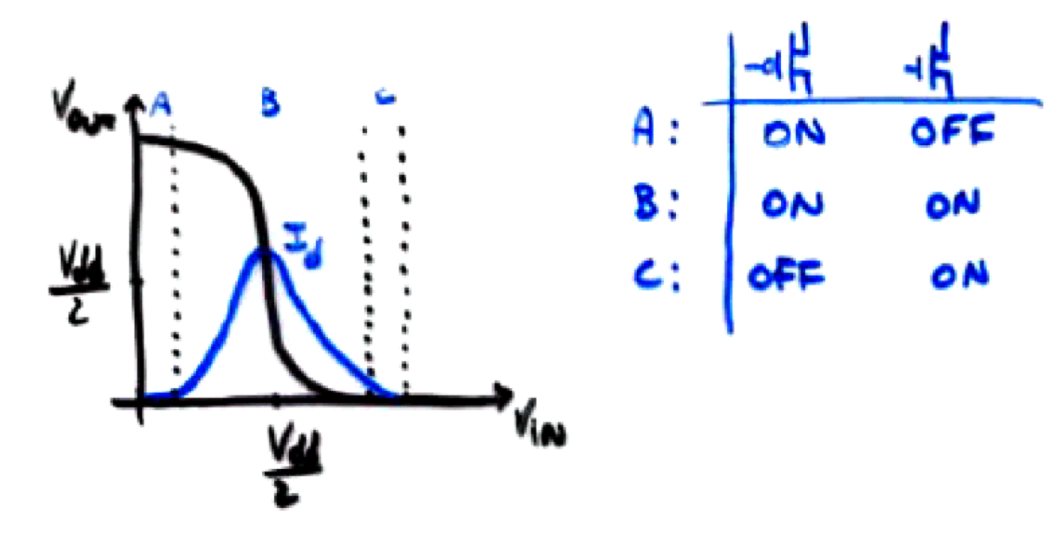
\includegraphics[width=.6\linewidth]{Figures/inverting_amplifier_power_consumption.PNG}
    \caption{The slow switching time of an inverting amplifier generates a large current flow from $V_{dd}$ to ground.}
    \label{fig:inverting_amplifier_power_consumption}
\end{figure}

\begin{figure}
    \centering
    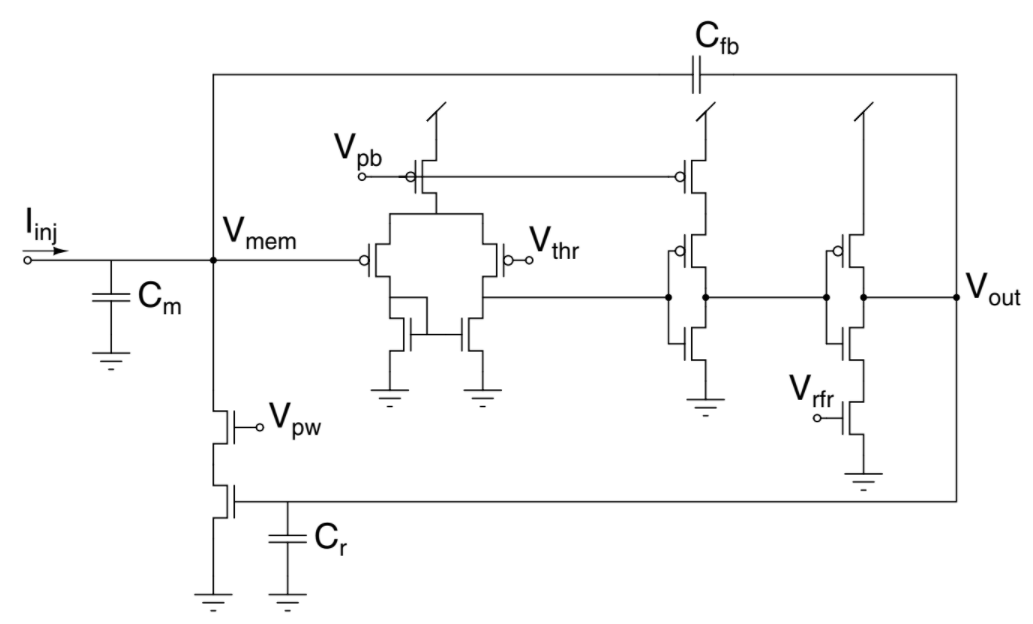
\includegraphics[width=\linewidth]{Figures/elaborate_if_neuron.PNG}
    \caption{A more elaborate circuit of an integrate-and-fire neuron.}
    \label{fig:elaborate_if_circuit}
\end{figure}